\documentclass[12pt]{article}
\usepackage[utf8]{inputenc} % allow utf-8 input
\usepackage[T1]{fontenc}    % use 8-bit T1 fonts
\usepackage{lmodern}
\usepackage{hyperref}       % hyperlinks  %[implicit=false, bookmarks=false]
\usepackage{url}            % simple URL typesetting
\usepackage{booktabs}       % professional-quality tables
\usepackage{amsfonts}       % blackboard math symbols
\usepackage{nicefrac}       % compact symbols for 1/2, etc.
\usepackage{microtype}      % microtypography
\usepackage[margin=1.0in]{geometry}

\usepackage{mathtools, amsmath, amssymb, amsthm, graphicx, verbatim}
%\usepackage[thmmarks, thref, amsthm]{ntheorem}
\usepackage{color}
\definecolor{darkblue}{rgb}{0.0,0.0,0.2}
\hypersetup{colorlinks,breaklinks,
            linkcolor=darkblue,urlcolor=darkblue,
            anchorcolor=darkblue,citecolor=darkblue}
\usepackage{wrapfig}
\usepackage{subcaption}
\usepackage[colorinlistoftodos,textsize=tiny]{todonotes} % need xargs for below
%\usepackage{accents}
\usepackage{bbm}
\usepackage{xspace}

\usetikzlibrary{calc}
\newcommand{\Comments}{1}
\newcommand{\mynote}[2]{\ifnum\Comments=1\textcolor{#1}{#2}\fi}
\newcommand{\mytodo}[2]{\ifnum\Comments=1%
  \todo[linecolor=#1!80!black,backgroundcolor=#1,bordercolor=#1!80!black]{#2}\fi}
\newcommand{\raf}[1]{\mynote{green}{[RF: #1]}}
\newcommand{\raft}[1]{\mytodo{green!20!white}{RF: #1}}
\newcommand{\jessie}[1]{\mynote{purple}{[JF: #1]}}
\newcommand{\jessiet}[1]{\mytodo{purple!20!white}{JF: #1}}
\newcommand{\bo}[1]{\mynote{blue}{[Bo: #1]}}
\newcommand{\botodo}[1]{\mytodo{blue!20!white}{[Bo: #1]}}
\ifnum\Comments=1               % fix margins for todonotes
  \setlength{\marginparwidth}{1in}
\fi


\newcommand{\reals}{\mathbb{R}}
\newcommand{\posreals}{\reals_{>0}}%{\reals_{++}}
\newcommand{\dom}{\mathrm{dom}}
\newcommand{\epi}{\text{epi}}
\newcommand{\relint}{\mathrm{relint}}
\newcommand{\prop}[1]{\Gamma[#1]}
\newcommand{\eliccts}{\mathrm{elic}_\mathrm{cts}}
\newcommand{\eliccvx}{\mathrm{elic}_\mathrm{cvx}}
\newcommand{\elicpoly}{\mathrm{elic}_\mathrm{pcvx}}
\newcommand{\elicembed}{\mathrm{elic}_\mathrm{embed}}

\newcommand{\cell}{\mathrm{cell}}

\newcommand{\abstain}[1]{\mathrm{abstain}_{#1}}
\newcommand{\mode}{\mathrm{mode}}

\newcommand{\simplex}{\Delta_\Y}

% alphabetical order, by convention
\newcommand{\C}{\mathcal{C}}
\newcommand{\D}{\mathcal{D}}
\newcommand{\E}{\mathbb{E}}
\newcommand{\F}{\mathcal{F}}
\newcommand{\I}{\mathcal{I}}
\newcommand{\R}{\mathcal{R}}
\newcommand{\U}{\mathcal{U}}
\newcommand{\X}{\mathcal{X}}
\newcommand{\Y}{\mathcal{Y}}

\newcommand{\risk}[1]{\underline{#1}}
\newcommand{\inprod}[2]{\langle #1, #2 \rangle}%\mathrm{int}(#1)}
\newcommand{\inter}[1]{\mathrm{int}(#1)}%\mathrm{int}(#1)}
%\newcommand{\expectedv}[3]{\overline{#1}(#2,#3)}
\newcommand{\expectedv}[3]{\E_{Y\sim{#3}} {#1}(#2,Y)}
\newcommand{\toto}{\rightrightarrows}
\newcommand{\strip}{\mathrm{strip}}
\newcommand{\trim}{\mathrm{trim}}
\newcommand{\fplc}{finite-piecewise-linear and convex\xspace} %xspace for use in text
\newcommand{\conv}{\mathrm{conv}}
\newcommand{\indopp}{\bar{\mathbbm{1}}}
\newcommand{\ones}{\mathbbm{1}}
\DeclarePairedDelimiter\ceil{\lceil}{\rceil}

\newcommand{\Ind}[1]{\mathbf{1}\{#1\}}

\DeclareMathOperator*{\argmax}{arg\,max}
\DeclareMathOperator*{\argmin}{arg\,min}
\DeclareMathOperator*{\arginf}{arg\,inf}
\DeclareMathOperator*{\sgn}{sgn}

\newtheorem{theorem}{Theorem}
\newtheorem{lemma}{Lemma}
\newtheorem{proposition}{Proposition}
\newtheorem{definition}{Definition}
\newtheorem{corollary}{Corollary}
\newtheorem{conjecture}{Conjecture}


\title{Embedding Dimension-- fixing a report}
\date{}

\begin{document}

\maketitle

\section*{Notation}
Let $\gamma:\simplex \toto \R$ be a finite, nondegenerate, elicitable property, i.e. $|\R| < \infty$ and $\gamma(p) \neq \emptyset$ for all $p \in \simplex$.

For $p \in \simplex$, we denote polytope $T(r,p) := \sum_{y \in \Y}p_y T(r,y)$, where summation is the Minkowski sum.

\section*{Background}
We know from Lambert 09 and 18 that the cells $\{\gamma_r\}_{r \in \R}$ form a power diagram, or equivalently, a Voronoi diagram restricted to $\simplex$.
This implies that each level set $\gamma_r$ is a convex polytope, and it has been established each polytope has both an $H$-representation (halfspace; written as matrix inequality) and a $V$-representation (vertex; written as the convex hull of a finite set of vertices).

We fix some report $r \in \R$ and focus on its level set $\gamma_r$.
Again, since $\gamma$ is a finite, elicitable property, we know that $\gamma_r$ is a convex polytope.
By existence of the $H$-representation of $\gamma_r$, we know there is a matrix $B^r \in \reals^{k \times n}$ and vector $b \in \reals^k$ so that $\gamma_r = \{p \in \simplex : B^r p \geq b\}$.
In fact, we can fix $b = \vec 0$, as we will show later by construction of $B^r$.
We will want to construct polytopes $T(r,p)$ that are Minkowski sums of a finite set of other polytopes.
We aim to construct $T$ so that $p \in \{p \in \simplex : B^r p \geq 0\} \iff \vec 0 \in \sum_y p_y T(r,y)$.
To do this, we characterize when $x \in T(r,p) := \sum_{y \in \Y} p_y T(r,y)$, later substituting $x = \vec 0$, where summation is the Minkowski sum.


For each face $F$ of $T(r,p)$, there is a unique decomposition of faces $F_y$ of $T(r,y)$ for each $y \in \Y$ such that $F = \sum_y F_y$.\jessie{EPFLTH Theorem 3.1.2}
Each of these faces share a normal $v$ by \jessie{EPFLTH Corollary 3.1.14}, where there is a face $F_y = \{x : vx = b_y\}$.
Then $x \in T(r,p) \implies v x \leq \sum_y p_y b_y$.
Substituting $x = 0$, we then see $0 \in T(r,p) \implies 0 \leq p_y b_y$ for all $y \in \Y$.
Letting $B^r$ be the matrix of vectors $b$ and taking $x = 0$, we observe the construction $\vec 0 \in T(r,p) \iff B^rp \geq \vec 0$ for all such matrices $B^r$ and $p \in \simplex$.
Thus, we can take $B^r$ to describe the level set $\gamma_r$.

In describing $\gamma_r$, since $\dom(\gamma) = \simplex$, it is worth asking if the constraints imposed by $\simplex$ can be assumed by the elicitability of $\gamma$, or if they need to additionally be built into the construction of $B^r$.
From my understanding, they can be assumed, since elicitability gives us a Voronoi diagram \emph{restricted to the simplex}: an equivalent definition to a Power Diagram.
By restricting to the simplex, we can focus on the cells of a Voronoi diagram, which are always convex polytopes.


\section*{Level sets to loss functions}
While having the property we want to work with is great, our end goal is to end up constructing a [probably polyhedral] loss function that elicits such a property.
We know there are two conditions that must be true in order for any loss $L$ to elicit $\gamma$: optimality and monotonicity.

These conditions are stated formally below, and justified in the following subsections.
\begin{theorem}[COLT paper Theorem approx 25]
A finite property is $d$-embeddable if and only if there exist polytopes $T(r,y)$ such that the following two conditions hold:
\begin{enumerate}
	\item (Monotonicity.) There exists an embedding $\varphi:\R \to \reals^d$ and a set of convex functions $\{L_y: \reals^d \to \reals_+\}_{y \in \Y}$ such that for all $y \in \Y$ and $r \in \R$, we have $T(r,y) = \partial_r L_y(\varphi(r))$.
	\item (Optimality.) For all $r \in \R$ and $p \in \simplex$, we have $r \in \gamma(p) \iff \vec 0 \in T(r,p)$.
\end{enumerate}
\end{theorem}

This gives us a characterization, although not a construction, of loss functions that elicit the desired property.
Our goal is to use this characterization to construct a loss function $L$ indirectly eliciting $\gamma$, where the link function is simply a restriction of reports.  (i.e. $L$ should embed $\ell$ eliciting $\gamma$.)

\subsection*{Monotonicity}
Given a finite, elicitable property $\gamma$, we know there is \emph{some} loss that elicits it.
The monotonicity condition prods us to ask what such a convex loss can look like.
For convex $L$ and $u \in \inter{\dom(L)}$, the subgradient set $\partial_r L_y(u)$ is closed and bounded\footnote{In B/V notes}; as a corollary of this fact and our monotonicity requirement\jessie{Assuming all embeddings map to the interior of the domain}, so must $T(r,y)$ be closed and bounded for all $r \in \R$ and $y \in \Y$; hence polytopes instead of polyhedra. 

%\jessie{Not in stated condition, but we want this as well.}
%In our mode example, consider distributions where $p_1 = p_2 > p_3$ for concreteness if needed.
%In this case, whatever loss function elicits the property must be flat (and minimized, by optimality) on $\conv{\{\varphi(1), \varphi(2)\}}$, so that the origin is in the subgradient sets of both $\inprod{L(\varphi(1))}{p}$ and $\inprod{L(\varphi(2))}{p}$.
%
%Moreover, we want ``adjacent'' reports to share a face of their subgradient sets for all $y \in \Y$, so that they share a face of their subgradient sets on the expected loss for the distributions where both are optimal.


\subsection*{Optimality}
The forward implication of the optimality condition makes sense once we think about the loss eliciting $\gamma$.
Since, in the monotonicity condition, we set $T(r,y) := \partial L_y(\varphi(r))$, then the embedded report must minimize the loss by elicitability, and therefore $\vec 0$ must be in the subgradient set.
Similarly, for the reverse implication, if $\vec 0 \in T(r,p)$ then we can see that $\varphi(r)$ minimizes the expected loss over $p$.
We can take Minkowski sums by the subdifferential sum rule\footnote{\url{https://maunamn.wordpress.com/8-the-subdifferential-sum-rule/}}, assuming $\varphi(r) \in \relint(\dom(L_y))$ for all $y \in \Y$.


This is a (finite) higher-dimensional generalization of the fact that a report $r$ is a minimizer of a function if and only if $\vec 0$ is in its subgradient set.



\section*{Construction}
We consider the subgradient sets of the loss we aim to construct, and try to relate the subgradient sets of embedded reports to the geometry of the property values.

Our embedding requirements depend on the existence of some polytopes $T(r,y)$ that simultaneously satisfy optimality and monotonicity requirements.
Our goal to construct such polytopes in the lowest dimension $d$ possible.

Since each $T(r,y)$ is a convex polytope, we know it there exists $V \in \reals^{k \times d}$ and $b \in \reals^k$ such that $T(r,y) = \{x \in \reals^d : Vx \leq b\}$.


Enforcing our optimality constraints brings us back to the $B^r$ matrix discussed earlier.
We aim to construct $T$ so that $r \in \gamma(p) \iff \vec 0 \in T(r,p)$ for all reports $r \in \R$ and $p \in \simplex$.
Consider that $r \in \gamma(p) \iff p \in \gamma_r$, and we chose $B^r$ so that $\gamma_r = \{p \in \simplex : B^rp \geq 0\}$.
Thus, we can re-write the condition as $p \in \{q \in \simplex : B^rq \geq 0\} \iff r \in \gamma(p) \iff \vec 0 \in T(r,p)$, stated for clarity below.
\begin{align*}
\forall p \in \simplex, \; B^r p \geq 0 &\iff \vec 0 \in T(r,p)
\end{align*}

In general, we consider the $H$-representation of $T(r,y) := \{x \in \reals^d : V^r x \leq b\}$ for some $V^r \in \reals^{k \times d}$ and $b \in \reals^k$.
\jessie{Question 3: How to find $V^r$?} 
As discussed earlier, in order to force optimality constraints to be satisfied, we designate $b$ to be the $y^{th}$ column of $B^r$ demonstrated by the construction above.

However, these are not the only constraints in constructing $T(r,y)$.
Since $T(r,y)$ becomes the subgradient of $L$ at the embedding of $r$, we also restrict that $T$ must be closed and bounded.
Thus, we ask how to properly restrict the construction of $T(r,y)$ so it is a polytope. \jessie{See Question 1}


\section*{Results}

Conditions on each $T(r,y)$ and $T(r,p)$ for all $p \in \simplex$:
\begin{enumerate}
	\item Closed and bounded (by monotonicity and subgradient characterization)
	\item Constructed with $B^r$ matrix (optimality)
	\item For all $p \in \gamma_r \cap \gamma_{r'}$, the polytopes $T(r,p)$ and $T(r',p)$ must share a face containing $\vec 0$. (monotonicity, but not as stated.)
	This suggests that the expected loss is flat on such distributions.
\end{enumerate}

One thought on restricting polytopes $T(r,y)$: for each $r \in \R$, consider the $R$ sets such that $\cap_{r' \in R} \gamma_{r'} \neq \emptyset$ and $r \in R$.
For all $p \in \cap_{r' \in R}\gamma_{r'}$, the polytopes $T(r',p)$ should share a face, possibly of a certain dimension.  (i.e. dim(level set) + dim(face) = n?) 

\section*{Questions}
\begin{enumerate}
	\item How to make the polyhedra $T(r,y)$ satisfying minimal optimality requirements be bounded? Do we do this by intersecting minimal $H$-rep with some polar, possibly $V^\circ$? 
	\item Can \emph{any} bounded polytopes $T(r,y)$ satisfying optimality and monotonicity constraints be $\partial L(r)_y$.  In other words, could the valid $T$ constructions characterize the polyhedral losses that embed $\gamma$?
	\item \jessie{Ask Nathan?} How to find $V^r$, given $B^r$ for each $r \in \R$?  Poly-time?
	\item Is there a framework where we construct $T(r,y)$ by going from H-reps to V-reps, to H-reps?  (It's computationally hard to calculate closed form of H-rep Minkowski sum, but we can just back and forth for closed polytopes in poly time.)
	\item How does duality play into all of this?  
\end{enumerate}

\bigskip \hrule \bigskip
\section*{Example: The mode}
Consider the mode with $n=3$, whose level sets are drawn in Figure~\ref{fig:mode-simplex}.
We will revisit this as a working example throughout in order to have something concrete to visualize.

\begin{figure}
	\centering
	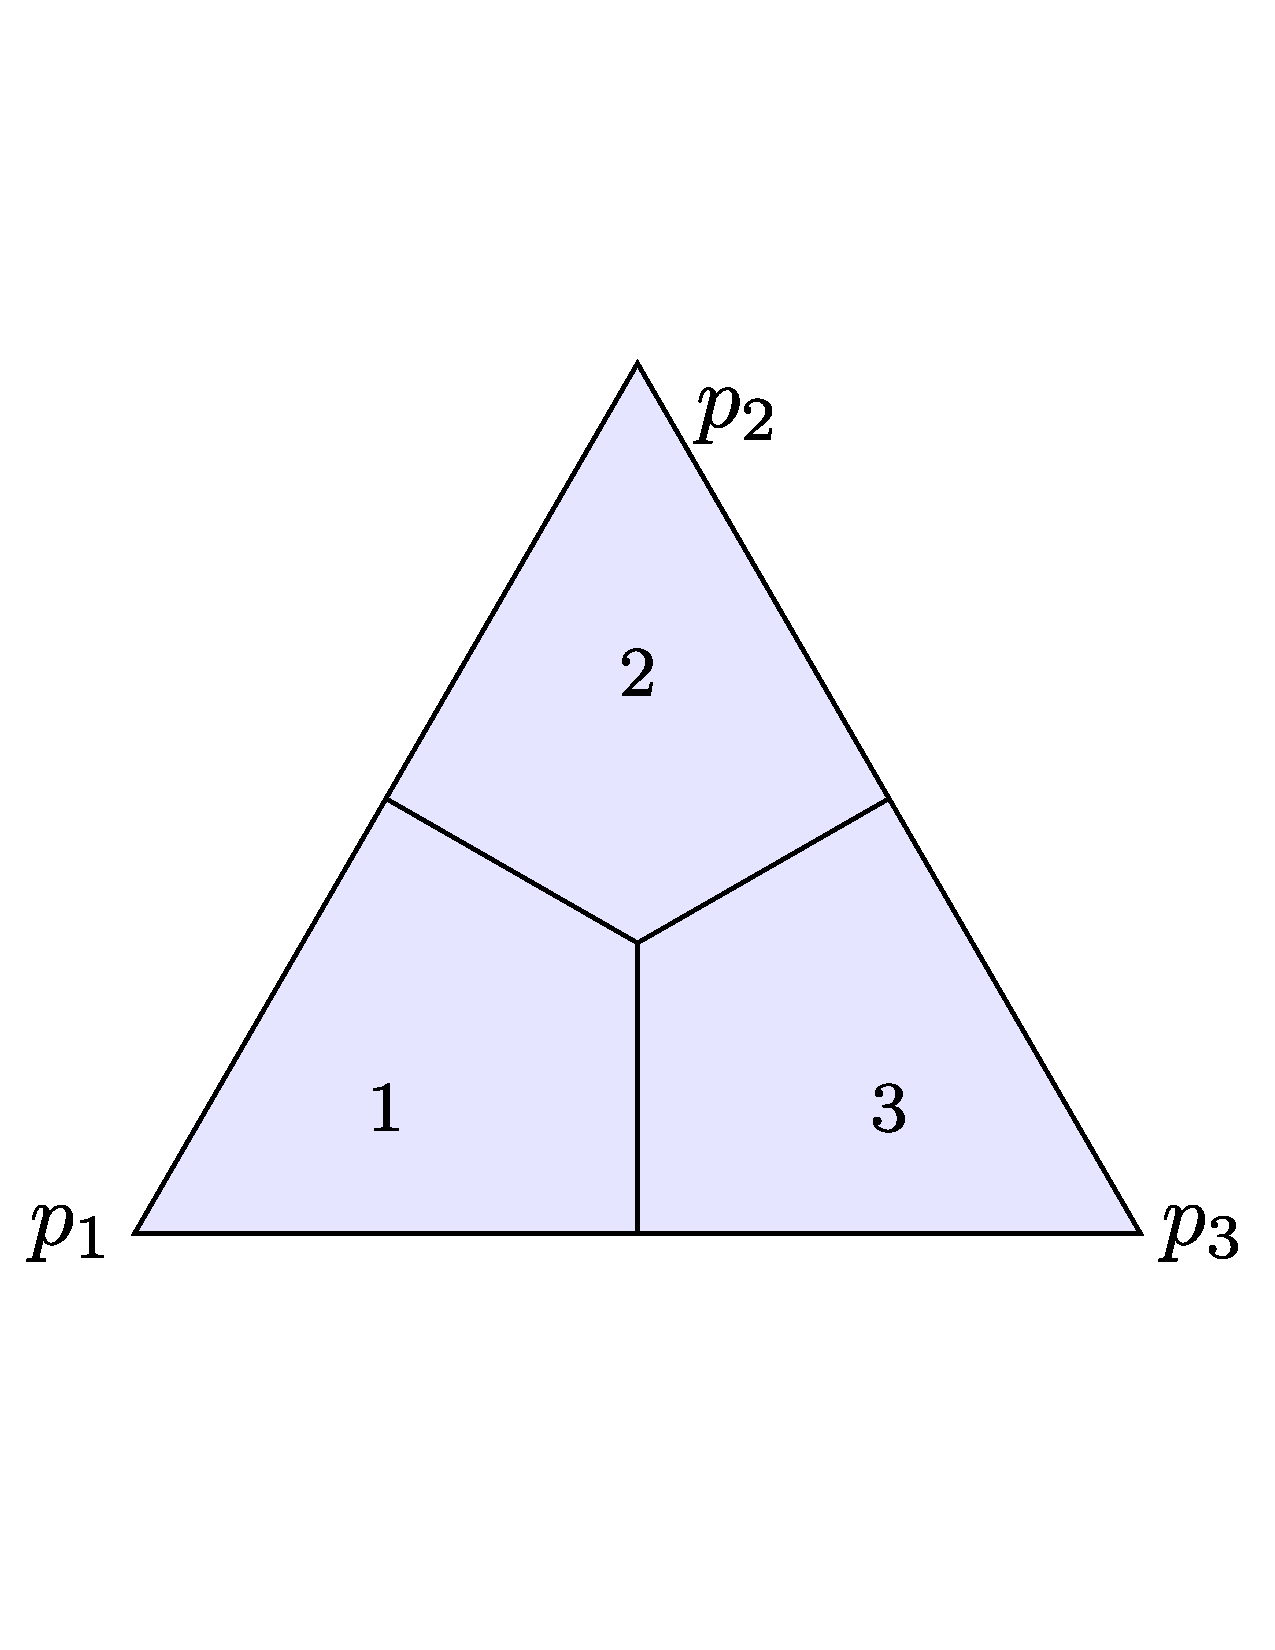
\includegraphics[width=0.5\linewidth]{figs/mode-simplex}
	\caption{Level sets of the mode $\gamma(p) = \argmax_y p_y$ with $n=3$.}
	\label{fig:mode-simplex}
\end{figure}

We can describe the cell $\gamma_1$ in one of two, nonequivalent, ways:
\[
\{p \in \simplex: 
\begin{bmatrix}
1 & -1 & 0\\
1 & 0 & -1
\end{bmatrix} \vec p \geq \vec 0 \}
\]
or
\[
\left\{p \in \reals^n: 
\begin{bmatrix}
1 & -1 & 0\\
1 & 0 & -1\\
0 & 1 & 0\\
0 & 0 & 1
\end{bmatrix} \vec p \geq \vec 0 \right\}
\].

These are nonequivalent since the latter doesn't include the simplex requirement that $\sum_y p_y = 1$; a constraint we cannot capture without changing the right side of the inequality to be nonzero.

However, since we can take $p \in \simplex$, we use the former formulation to describe $\gamma_1$.
If one observes that $1$ is in the argmax if and only if $p_1 \geq p_2$ and $p_1 \geq p_3$, we can see these conditions correspond to the first and second rows of the $B^1$ matrix, respectively.

\end{document}
%%% Local Variables:
%%% mode: latex
%%% TeX-master: t
%%% End:
